\documentclass[landscape]{article}

\usepackage{tikz}
\usetikzlibrary{mindmap,trees,backgrounds}
\usepackage[paperwidth=25cm,paperheight=22cm,left=1cm,top=1cm]{geometry}

\begin{document}
\pagestyle{empty}
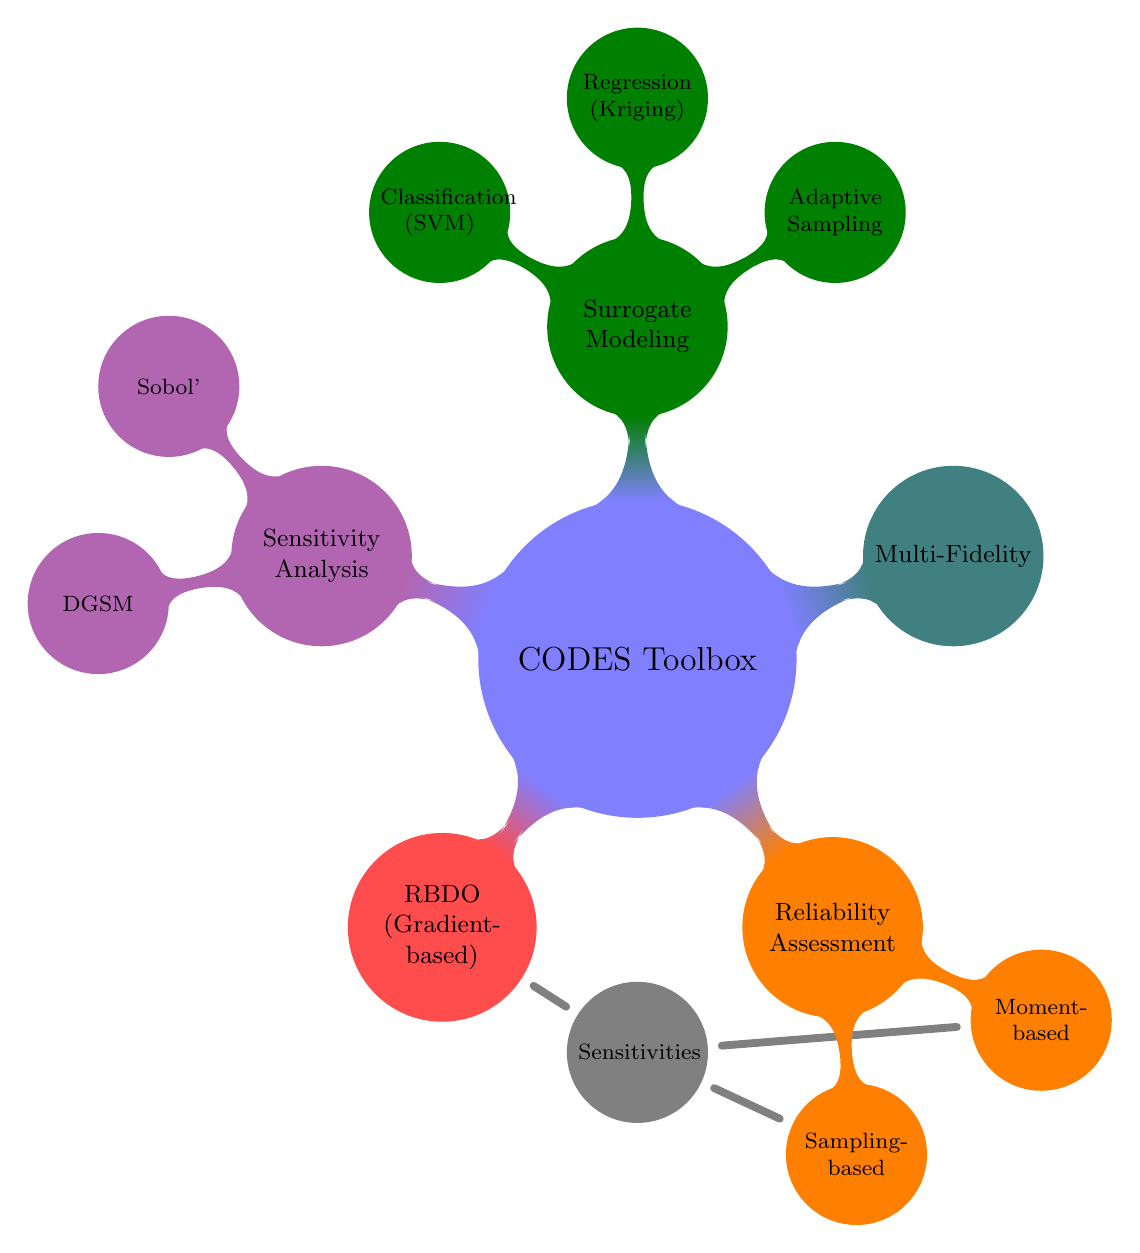
\begin{tikzpicture}[mindmap,concept color=blue!50,text=black,
					level 1 concept/.append style={level distance=120,sibling angle=72}]
	\node[concept] {CODES Toolbox}
	[clockwise from=18]
	child[concept color=blue!50!green!50!gray] {
		node[concept]{Multi-Fidelity}
	}
	child[concept color=orange] {
		node[concept] {Reliability Assessment}
		[clockwise from=-24]
		child {
			node[concept](moment){Moment-based}
		}
		child {
			node[concept](sampling){Sampling-based}
		}
	}
	child[concept color=red!70] {
		node[concept] (rbdo) {RBDO (Gradient-based)}
	}
	child[concept color=violet!60] {
		node[concept]{Sensitivity Analysis}
		[clockwise from=192]
		child {
			node[concept]{DGSM}
		}
		child {
			node[concept]{Sobol'}
		}
	}
	child[concept color=green!50!black] {
		node[concept] {Surrogate Modeling}
		[clockwise from=150]
		child {
			node[concept] {Classification (SVM)}
		}
		child {
			node[concept] {Regression (Kriging)}
		}
		child {
			node[concept] {Adaptive Sampling}
		}
	}
	node[extra concept] (sensitivities) at (0,-5) {Sensitivities};
	\begin{pgfonlayer}{background}
	\draw [concept connection]
		(moment) edge (sensitivities)
		(sampling) edge (sensitivities)
		(rbdo) edge (sensitivities);
	\end{pgfonlayer}
\end{tikzpicture}
\end{document}